% Copyright (c) 2013 Alexander Bluhm <bluhm@openbsd.org>
%
% Permission to use, copy, modify, and distribute this software for any
% purpose with or without fee is hereby granted, provided that the above
% copyright notice and this permission notice appear in all copies.
%
% THE SOFTWARE IS PROVIDED "AS IS" AND THE AUTHOR DISCLAIMS ALL WARRANTIES
% WITH REGARD TO THIS SOFTWARE INCLUDING ALL IMPLIED WARRANTIES OF
% MERCHANTABILITY AND FITNESS. IN NO EVENT SHALL THE AUTHOR BE LIABLE FOR
% ANY SPECIAL, DIRECT, INDIRECT, OR CONSEQUENTIAL DAMAGES OR ANY DAMAGES
% WHATSOEVER RESULTING FROM LOSS OF USE, DATA OR PROFITS, WHETHER IN AN
% ACTION OF CONTRACT, NEGLIGENCE OR OTHER TORTIOUS ACTION, ARISING OUT OF
% OR IN CONNECTION WITH THE USE OR PERFORMANCE OF THIS SOFTWARE.

\documentclass[14pt]{beamer}
\usetheme{Frankfurt}
\usepackage{tikz}
\author{Alexander Bluhm}
\title{Zero-Copy Socket Splicing}
\institute{\url{bluhm@openbsd.org}}
\date{Sunday, 29. September 2013}

\begin{document}

\begin{frame}
\titlepage
\end{frame}

\begin{frame}{Agenda}
\tableofcontents
\end{frame}

\section{Motivation}

\begin{frame}{Agenda}
\tableofcontents[currentsection]
\end{frame}

\begin{frame}{Application Level Gateway}
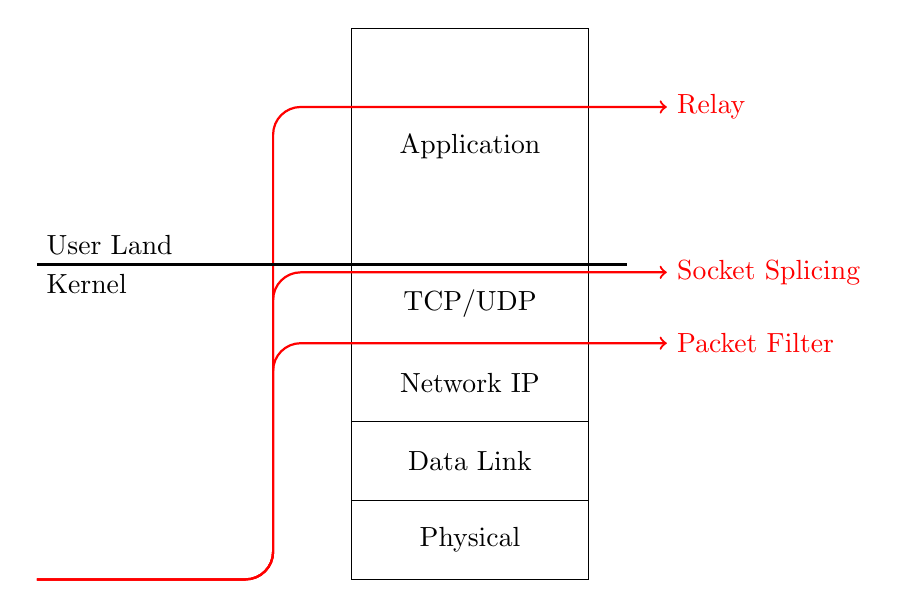
\begin{tikzpicture}
\draw (-1,0) rectangle +(3,1) node(l1) [midway] {Physical};
\draw (-1,1) rectangle +(3,1) node(l2) [midway] {Data Link};
\draw (-1,2) rectangle +(3,1) node(l3) [midway] {Network IP};
\draw (-1,3) rectangle +(3,1) node(l4) [midway] {TCP/UDP};
\draw (-1,4) rectangle +(3,3) node(l5) [midway] {Application};
\begin{scope}[->,rounded corners=10,thick,red]
\draw (-5,0) -- ++(3,0) -- ++(0,3) -- ++(5,0) node [right] {Packet Filter};
\draw (-5,0) -- ++(3,0) -- ++(0,6) -- ++(5,0) node [right] {Relay};
\end{scope}
\draw[thick] (-5,4) node(context) {} -- +(7.5,0);
\node [below right] at (context) {Kernel};
\node [above right] at (context) {User Land};
\begin{scope}[->,rounded corners=10,thick,red]
\draw (-5,0) -- ++(3,0) -- ++(0,3.9) -- ++(5,0) node [right] {Socket Splicing};
\end{scope}
\end{tikzpicture}
\end{frame}

\begin{frame}{Persistent HTTP Filtering}
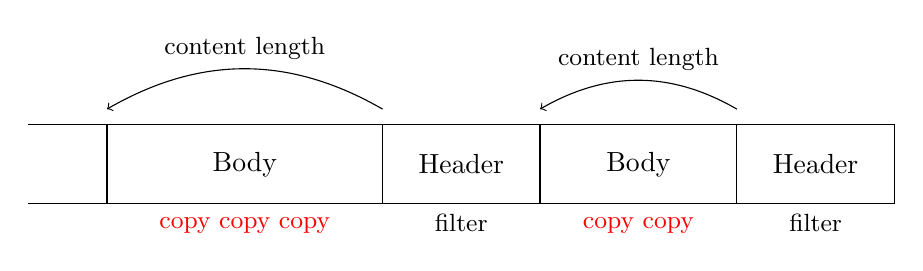
\begin{tikzpicture}
\draw
    (0,0) -- ++(1,0) -- ++(0,1) -- +(-1,0)
    ++(0,-1)  rectangle ++(3.5,1) node (b2) [midway] {Body}
    { [current point is local] ++(0,.2) edge [->,bend right] 
	node [above,font=\small] {content length} ++(-3.5,0) }
    ++(0,-1)  rectangle ++(2,1)   node (h2) [midway] {Header}
    ++(0,-1)  rectangle ++(2.5,1) node (b1) [midway] {Body}
    { [current point is local] ++(0,.2) edge [->,bend right] 
	node [above,font=\small] {content length} ++(-2.5,0) }
    ++(0,-1)  rectangle ++(2,1)   node (h1) [midway] {Header};
\path
    (node cs:name=b2,anchor=south) +(0,-.5) node [font=\small,red]
	{copy copy copy}
    (node cs:name=h2,anchor=south) +(0,-.5) node [font=\small] {filter}
    (node cs:name=b1,anchor=south) +(0,-.5) node [font=\small,red] {copy copy}
    (node cs:name=h1,anchor=south) +(0,-.5) node [font=\small] {filter};
\end{tikzpicture}
\end{frame}

\begin{frame}{HTTP Socket Splicing}
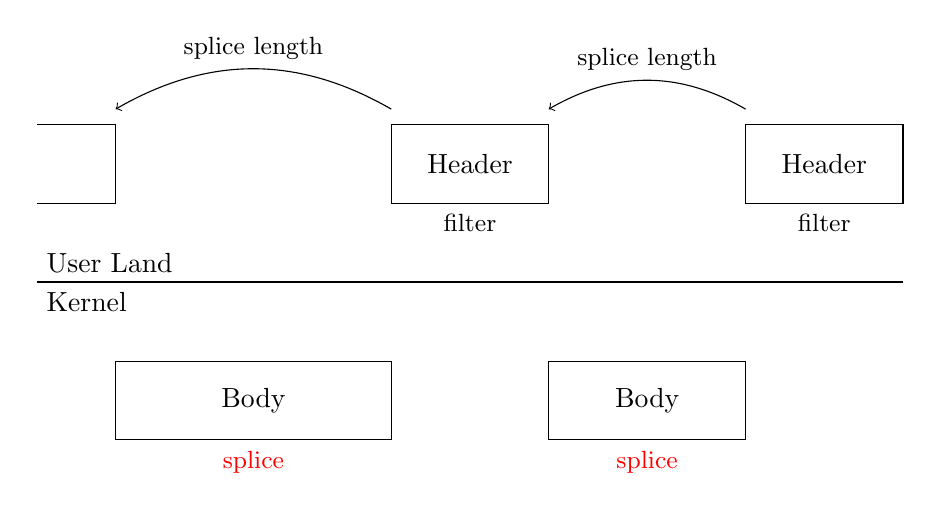
\begin{tikzpicture}
\draw
    (0,+1) -- ++(1,0) -- ++(0,1) -- +(-1,0)
    ++(0,-4)  rectangle ++(3.5,1) node (b2) [midway] {Body}
    { [current point is local] ++(0,3.2) edge [->,bend right] 
	node [above,font=\small] {splice length} ++(-3.5,0) }
    ++(0,+2)  rectangle ++(2,1)   node (h2) [midway] {Header}
    ++(0,-4)  rectangle ++(2.5,1) node (b1) [midway] {Body}
    { [current point is local] ++(0,3.2) edge [->,bend right] 
	node [above,font=\small] {splice length} ++(-2.5,0) }
    ++(0,+2)  rectangle ++(2,1)   node (h1) [midway] {Header};
\path
    (node cs:name=b2,anchor=south) +(0,-.5) node [font=\small,red] {splice}
    (node cs:name=h2,anchor=south) +(0,-.5) node [font=\small] {filter}
    (node cs:name=b1,anchor=south) +(0,-.5) node [font=\small,red] {splice}
    (node cs:name=h1,anchor=south) +(0,-.5) node [font=\small] {filter};
\draw[thick] (0,0) node(context) {} -- +(11,0);
\node [below right] at (context) {Kernel};
\node [above right] at (context) {User Land};
\end{tikzpicture}
\end{frame}

\section{Kernel MBuf}

\begin{frame}{Agenda}
\tableofcontents[currentsection]
\end{frame}

\begin{frame}{MBuf Data}
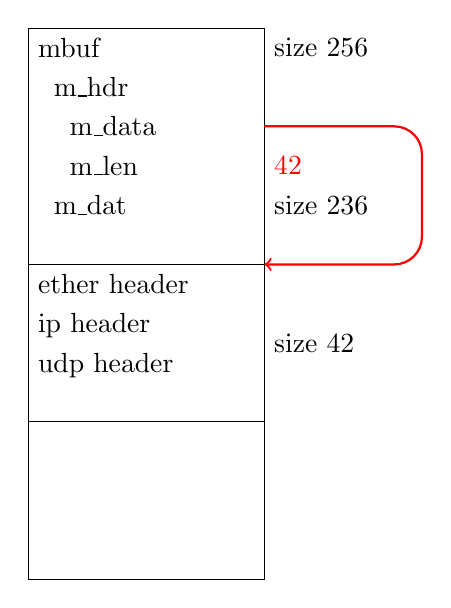
\begin{tikzpicture}
\draw
      ( 0  , 0  ) rectangle +(3,-7)
    ++( 0  , 0  ) node [below right] (mbuf)    {mbuf}
    ++(  .2,- .5) node [below right]           {m\_hdr}
    ++(  .2,- .5) node [below right] (mdata)   {m\_data}
    ++( 0  ,- .5) node [below right] (mlen)    {m\_len}
    ++(- .2,- .5) node [below right] (mdat)    {m\_dat}
      ( 0  ,-3  ) -- +(3,0)
    ++( 0  , 0  ) node [below right] {ether header}
    ++( 0  ,- .5) node [below right] {ip header}
    ++( 0  ,- .5) node [below right] {udp header}
      ( 0  ,-5  ) -- +(3,0);
\path
    (mbuf    -| 3,0) node [right] {size 256}
    (mlen    -| 3,0) node [right,red] {42}
    (mdat    -| 3,0) node [right] {size 236}
      ( 3  ,-4  )    node [right] {size 42};
\draw[->,rounded corners=10,thick,red]
    (mdata   -| 3,0) -| (5,-3) -- (3,-3);
\end{tikzpicture}
\end{frame}

\begin{frame}{MBuf Data Chaining}
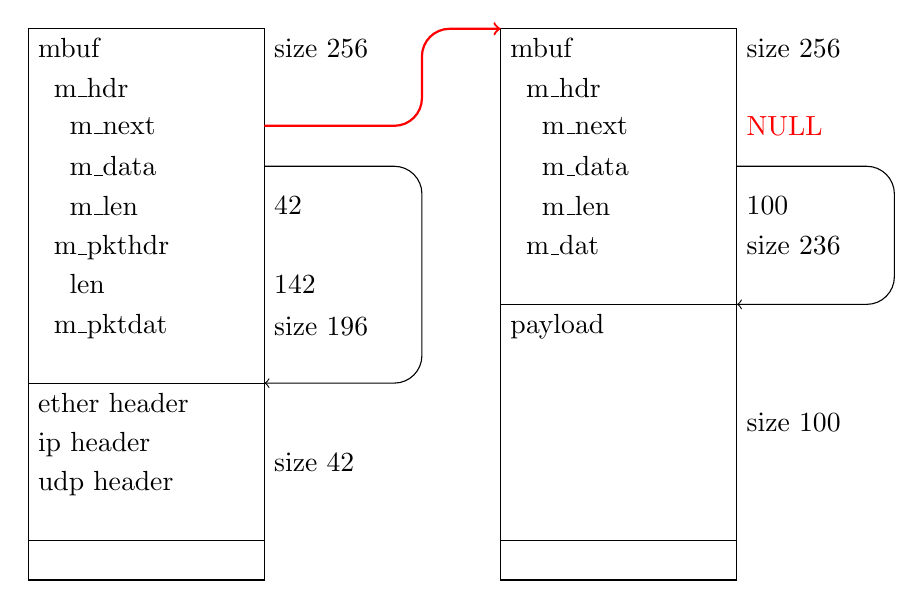
\begin{tikzpicture}
\draw
      ( 0  , 0  ) rectangle +(3,-7)
    ++( 0  , 0  ) node [below right] (mbuf0)    {mbuf}
    ++(  .2,- .5) node [below right]            {m\_hdr}
    ++(  .2,- .5) node [below right] (mnext0)   {m\_next}
    ++( 0  ,- .5) node [below right] (mdata0)   {m\_data}
    ++( 0  ,- .5) node [below right] (mlen0)    {m\_len}
    ++(- .2,- .5) node [below right]            {m\_pkthdr}
    ++(  .2,- .5) node [below right] (len0)     {len}
    ++(- .2,- .5) node [below right] (mpktdat0) {m\_pktdat}
      ( 0  ,-4.5) -- +(3,0)
    ++( 0  , 0  ) node [below right] {ether header}
    ++( 0  ,- .5) node [below right] {ip header}
    ++( 0  ,- .5) node [below right] {udp header}
      ( 0  ,-6.5) -- +(3,0);
\path
    (mbuf0    -| 3,0) node [right] {size 256}
    (mlen0    -| 3,0) node [right] {42}
    (len0     -| 3,0) node [right] {142}
    (mpktdat0 -| 3,0) node [right] {size 196}
      ( 3  ,-5.5)     node [right] {size 42};
\draw[->,rounded corners=10]
    (mdata0   -| 3,0) -| (5,-4.5) -- (3,-4.5);

\draw
      ( 6  , 0  ) rectangle +(3,-7)
    ++( 0  , 0  ) node [below right] (mbuf)    {mbuf}
    ++(  .2,- .5) node [below right]           {m\_hdr}
    ++(  .2,- .5) node [below right] (mnext)   {m\_next}
    ++( 0  ,- .5) node [below right] (mdata)   {m\_data}
    ++( 0  ,- .5) node [below right] (mlen)    {m\_len}
    ++(- .2,- .5) node [below right] (mdat)    {m\_dat}
      ( 6  ,-3.5  ) -- +(3,0)
    ++( 0  , 0  ) node [below right] {payload}
      ( 6  ,-6.5) -- +(3,0);
\path
    (mbuf    -| 9,0) node [right] {size 256}
    (mnext   -| 9,0) node [right,red] {NULL}
    (mlen    -| 9,0) node [right] {100}
    (mdat    -| 9,0) node [right] {size 236}
      ( 9  ,-5  )    node [right] {size 100};
\draw[->,rounded corners=10]
    (mdata   -| 9,0) -| (11,-3.5) -- (9,-3.5);

\draw[->,rounded corners=10,thick,red]
    (mnext0   -| 3,0) -| (5, 0  ) -- (6,0);
\end{tikzpicture}
\end{frame}

\begin{frame}{MBuf Packet Chaining}
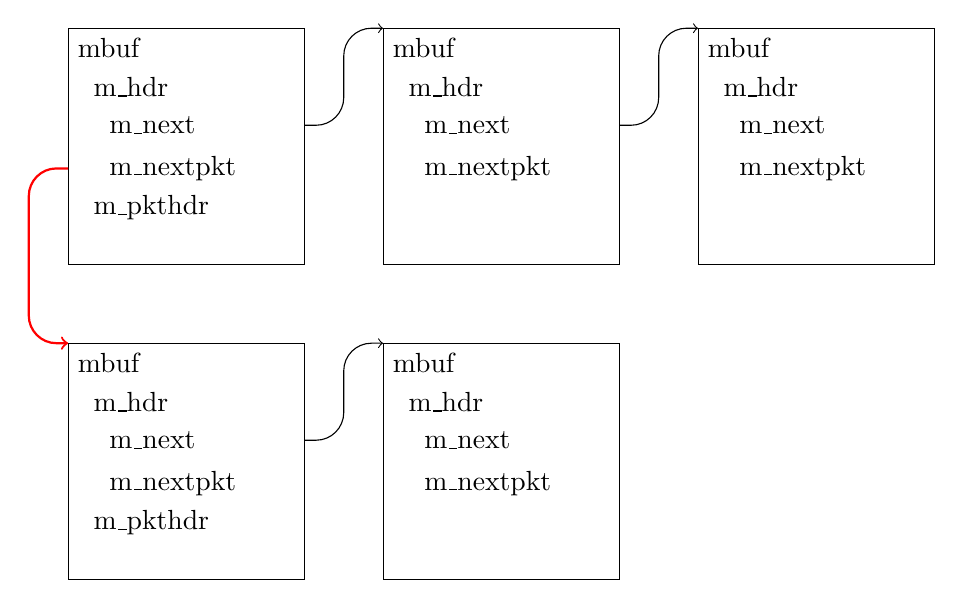
\begin{tikzpicture}
\draw
      ( 0  , 0  ) rectangle +(3,-3)
    ++( 0  , 0  ) node [below right] (mbuf00)     {mbuf}
    ++(  .2,- .5) node [below right]              {m\_hdr}
    ++(  .2,- .5) node [below right] (mnext00)    {m\_next}
    ++( 0  ,- .5) node [below right] (mnextpkt00) {m\_nextpkt}
    ++(- .2,- .5) node [below right]              {m\_pkthdr};
\draw
      ( 4  , 0  ) rectangle +(3,-3)
    ++( 0  , 0  ) node [below right] (mbuf01)     {mbuf}
    ++(  .2,- .5) node [below right]              {m\_hdr}
    ++(  .2,- .5) node [below right] (mnext01)    {m\_next}
    ++( 0  ,- .5) node [below right] (mnextpkt01) {m\_nextpkt};
\draw
      ( 8  , 0  ) rectangle +(3,-3)
    ++( 0  , 0  ) node [below right] (mbuf02)     {mbuf}
    ++(  .2,- .5) node [below right]              {m\_hdr}
    ++(  .2,- .5) node [below right] (mnext02)    {m\_next}
    ++( 0  ,- .5) node [below right] (mnextpkt02) {m\_nextpkt};
\draw[->,rounded corners=10]
    (mnext00 -| 3,0) -| (3.5,0) -- (4,0);
\draw[->,rounded corners=10]
    (mnext01 -| 7,0) -| (7.5,0) -- (8,0);

\draw
      ( 0  ,-4  ) rectangle +(3,-3)
    ++( 0  , 0  ) node [below right] (mbuf10)     {mbuf}
    ++(  .2,- .5) node [below right]              {m\_hdr}
    ++(  .2,- .5) node [below right] (mnext10)    {m\_next}
    ++( 0  ,- .5) node [below right] (mnextpkt10) {m\_nextpkt}
    ++(- .2,- .5) node [below right]              {m\_pkthdr};
\draw
      ( 4  ,-4  ) rectangle +(3,-3)
    ++( 0  , 0  ) node [below right] (mbuf11)     {mbuf}
    ++(  .2,- .5) node [below right]              {m\_hdr}
    ++(  .2,- .5) node [below right] (mnext11)    {m\_next}
    ++( 0  ,- .5) node [below right] (mnextpkt11) {m\_nextpkt};
\draw[->,rounded corners=10]
    (mnext10 -| 3,-4) -| (3.5,-4) -- (4,-4);
\draw[->,rounded corners=10,thick,red]
    (mnextpkt00 -| 0,0) -| (-.5,-4) -- (0,-4);
\end{tikzpicture}
\end{frame}

\begin{frame}{MBuf Cluster}
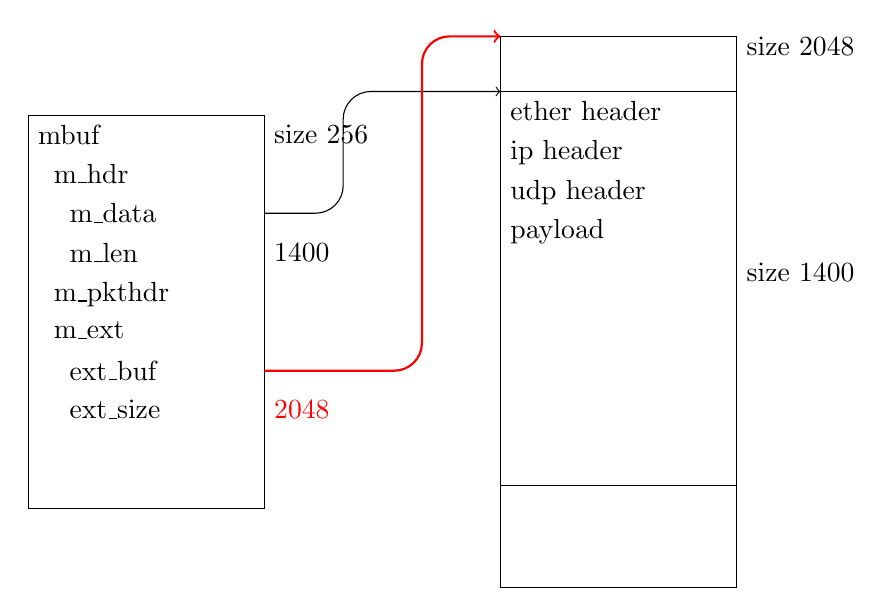
\begin{tikzpicture}
\draw
      ( 0  ,-1  ) rectangle +(3,-5)
    ++( 0  , 0  ) node [below right] (mbuf)    {mbuf}
    ++(  .2,- .5) node [below right]           {m\_hdr}
    ++(  .2,- .5) node [below right] (mdata)   {m\_data}
    ++( 0  ,- .5) node [below right] (mlen)    {m\_len}
    ++(- .2,- .5) node [below right]           {m\_pkthdr}
    ++( 0  ,- .5) node [below right]           {m\_ext}
    ++(  .2,- .5) node [below right] (extbuf)  {ext\_buf}
    ++( 0  ,- .5) node [below right] (extsize) {ext\_size};
\path
    (mbuf    -| 3,0) node [right] {size 256}
    (mlen    -| 3,0) node [right] {1400}
    (extsize -| 3,0) node [right,red] {2048};

\draw
      ( 6  , 0  ) rectangle +(3,-7)
    ++( 0  , 0  ) node [below right] (mcl)    {}
      ( 6  ,-.7 ) -- +(3,0)
    ++( 0  , 0  ) node [below right] {ether header}
    ++( 0  ,- .5) node [below right] {ip header}
    ++( 0  ,- .5) node [below right] {udp header}
    ++( 0  ,- .5) node [below right] {payload}
      ( 6  ,-5.7) -- +(3,0);
\path
    (mcl    -| 9,0) node [right] {size 2048}
      ( 9  ,  -3  ) node [right] {size 1400};
\draw[->,rounded corners=10]
    (mdata  -| 3,0) -| (4,-.7) -- (6,-.7);
\draw[->,rounded corners=10,thick,red]
    (extbuf -| 3,0) -| (5,0) -- (6,0);
\end{tikzpicture}
\end{frame}

\begin{frame}{MBuf Cluster Copy}
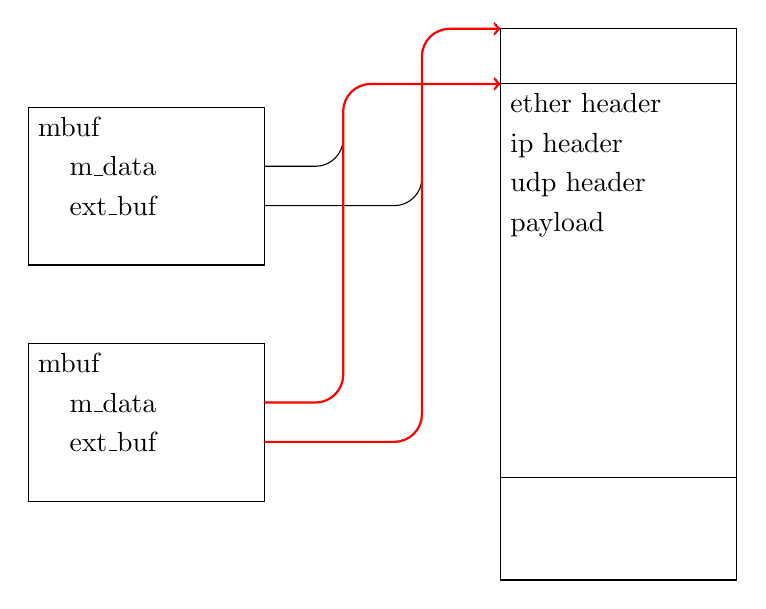
\begin{tikzpicture}
\draw
      ( 0  ,-1  ) rectangle +(3,-2)
    ++( 0  , 0  ) node [below right] (mbuf0)    {mbuf}
    ++(  .4,- .5) node [below right] (mdata0)   {m\_data}
    ++( 0  ,- .5) node [below right] (extbuf0)  {ext\_buf};

\draw
      ( 0  ,-4  ) rectangle +(3,-2)
    ++( 0  , 0  ) node [below right] (mbuf1)    {mbuf}
    ++(  .4,- .5) node [below right] (mdata1)   {m\_data}
    ++( 0  ,- .5) node [below right] (extbuf1)  {ext\_buf};

\draw
      ( 6  , 0  ) rectangle +(3,-7)
    ++( 0  , 0  ) node [below right] (mcl)    {}
      ( 6  ,-.7 ) -- +(3,0)
    ++( 0  , 0  ) node [below right] {ether header}
    ++( 0  ,- .5) node [below right] {ip header}
    ++( 0  ,- .5) node [below right] {udp header}
    ++( 0  ,- .5) node [below right] {payload}
      ( 6  ,-5.7) -- +(3,0);
\draw[->,rounded corners=10]
    (mdata0  -| 3,0) -| (4,-.7) -- (6,-.7);
\draw[->,rounded corners=10]
    (extbuf0 -| 3,0) -| (5,0) -- (6,0);
\draw[->,rounded corners=10,thick,red]
    (mdata1  -| 3,0) -| (4,-.7) -- (6,-.7);
\draw[->,rounded corners=10,thick,red]
    (extbuf1 -| 3,0) -| (5,0) -- (6,0);
\end{tikzpicture}
\end{frame}

\section{Packet Processing}

\begin{frame}{Agenda}
\tableofcontents[currentsection]
\end{frame}

\begin{frame}{Packet Input}
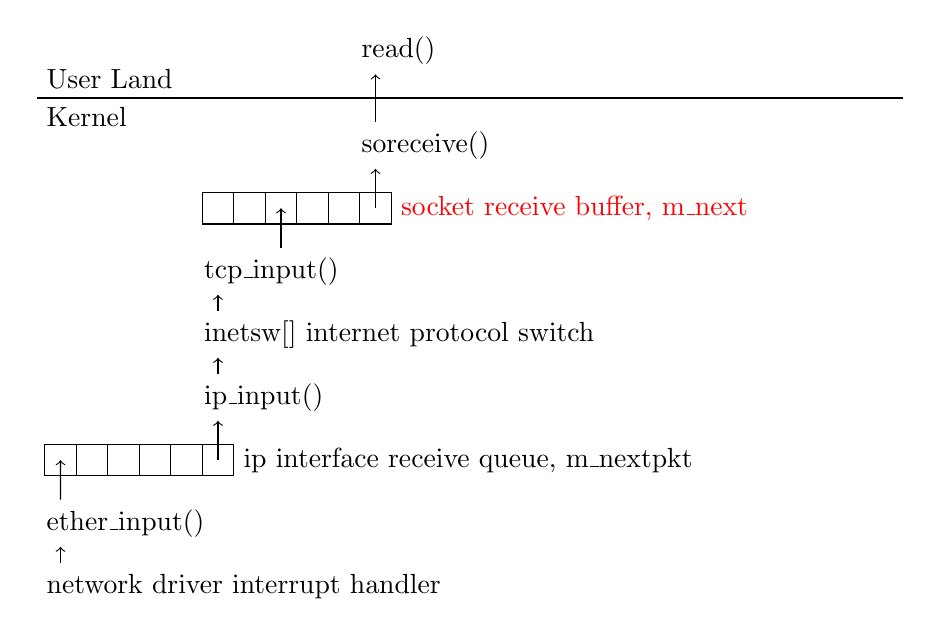
\begin{tikzpicture}
\draw (0,0)
    node (ni) [right] {network driver interrupt handler} ++(0,.8)
    node (ei) [right] {ether\_input()} ++(.1,.6)
    rectangle ++(.4,.4) rectangle ++(.4,-.4)
    rectangle ++(.4,.4) rectangle ++(.4,-.4)
    rectangle ++(.4,.4) rectangle ++(.4,-.4) ++(0,.2)
    node (rq) [right] {ip interface receive queue, m\_nextpkt} ++(-.5,.8)
    node (ii) [right] {ip\_input()} ++(0,.8)
    node (ps) [right] {inetsw[] internet protocol switch} ++(0,.8)
    node (ti) [right] {tcp\_input()} ++(.1,.6)
    rectangle ++(.4,.4) rectangle ++(.4,-.4)
    rectangle ++(.4,.4) rectangle ++(.4,-.4)
    rectangle ++(.4,.4) rectangle ++(.4,-.4) ++(0,.2)
    node (rb) [right,red] {socket receive buffer, m\_next} ++(-.5,.8)
    node (sr) [right] {soreceive()} ++(0,1.2)
    node (rd)  [right] {read()};

\path (node cs:name=ni,anchor=west) +(.3,.3) coordinate (nio) {};
\path (node cs:name=ei,anchor=west) +(.3,-.3) coordinate (eii) {};
\draw[->] (nio) -- (eii);
\path (node cs:name=ei,anchor=west) +(.3,.3) coordinate (eio) {};
\path (node cs:name=rq,anchor=west) +(-.2-5*.4,0) coordinate (rqi) {};
\draw[->] (eio) -- (rqi);
\path (node cs:name=rq,anchor=west) +(-.2,0) coordinate (rqo) {};
\path (node cs:name=ii,anchor=west) +(.3,-.3) coordinate (iii) {};
\draw[->] (rqo) -- (iii);
\path (node cs:name=ii,anchor=west) +(.3,.3) coordinate (iio) {};
\path (node cs:name=ps,anchor=west) +(.3,-.3) coordinate (psi) {};
\draw[->] (iio) -- (psi);
\path (node cs:name=ps,anchor=west) +(.3,.3) coordinate (pso) {};
\path (node cs:name=ti,anchor=west) +(.3,-.3) coordinate (tii) {};
\draw[->] (pso) -- (tii);
\path (node cs:name=ti,anchor=west) +(.3+2*.4,.3) coordinate (tio) {};
\path (node cs:name=rb,anchor=west) +(-.2-3*.4,0) coordinate (rbi) {};
\draw[->] (tio) -- (rbi);
\path (node cs:name=rb,anchor=west) +(-.2,0) coordinate (rbo) {};
\path (node cs:name=sr,anchor=west) +(.3,-.3) coordinate (sri) {};
\draw[->] (rbo) -- (sri);
\path (node cs:name=sr,anchor=west) +(.3,.3) coordinate (sro) {};
\path (node cs:name=rd,anchor=west) +(.3,-.3) coordinate (rdi) {};
\draw[->] (sro) -- (rdi);

\draw[thick] (rdi -| 0,0) ++(0,-.3) node (context) {} -- +(11,0);
\node [below right] at (context) {Kernel};
\node [above right] at (context) {User Land};
\end{tikzpicture}
\end{frame}

\begin{frame}{Packet Output}
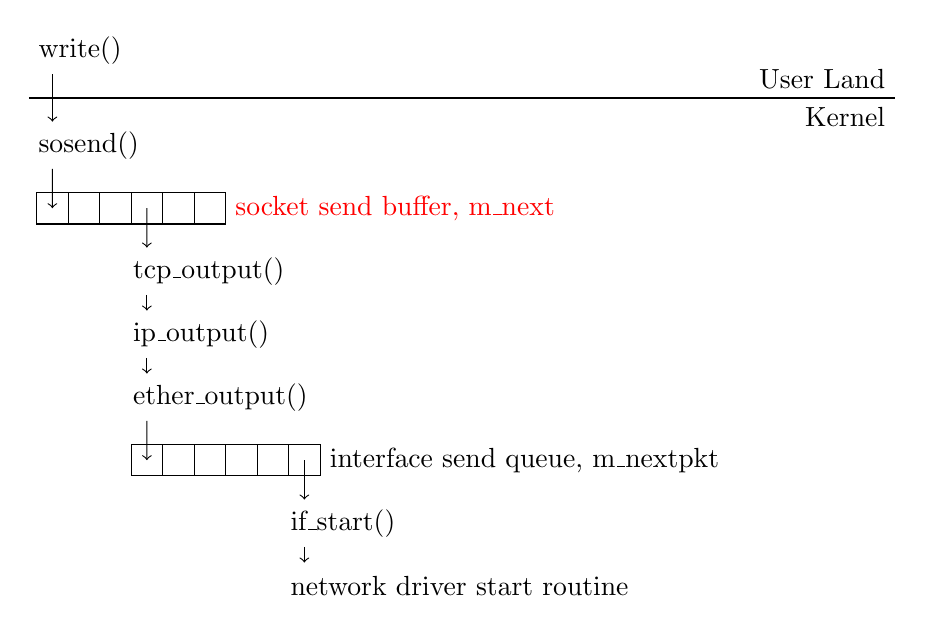
\begin{tikzpicture}
\draw (0,0)
    node (wr) [right] {write()} ++(0,-1.2)
    node (ss) [right] {sosend()} ++(.1,-.6)
    rectangle ++(.4,-.4) rectangle ++(.4,.4)
    rectangle ++(.4,-.4) rectangle ++(.4,.4)
    rectangle ++(.4,-.4) rectangle ++(.4,.4) ++(0,-.2)
    node (sb) [right,red] {socket send buffer, m\_next} ++(-1.3,-.8)
    node (to) [right] {tcp\_output()} ++(0,-.8)
    node (io) [right] {ip\_output()} ++(0,-.8)
    node (eo) [right] {ether\_output()} ++(.1,-.6)
    rectangle ++(.4,-.4) rectangle ++(.4,.4)
    rectangle ++(.4,-.4) rectangle ++(.4,.4)
    rectangle ++(.4,-.4) rectangle ++(.4,.4) ++(0,-.2)
    node (sq) [right] {interface send queue, m\_nextpkt} ++(-.5,-.8)
    node (is) [right] {if\_start()} ++(0,-.8)
    node (ns) [right] {network driver start routine};

\path (node cs:name=wr,anchor=west) +(.3,-.3) coordinate (wro) {};
\path (node cs:name=ss,anchor=west) +(.3,.3) coordinate (ssi) {};
\draw[->] (wro) -- (ssi);
\path (node cs:name=ss,anchor=west) +(.3,-.3) coordinate (sso) {};
\path (node cs:name=sb,anchor=west) +(-.2-5*.4,0) coordinate (sbi) {};
\draw[->] (sso) -- (sbi);
\path (node cs:name=sb,anchor=west) +(-.2-2*.4,0) coordinate (sbo) {};
\path (node cs:name=to,anchor=west) +(.3,.3) coordinate (toi) {};
\draw[->] (sbo) -- (toi);
\path (node cs:name=to,anchor=west) +(.3,-.3) coordinate (too) {};
\path (node cs:name=io,anchor=west) +(.3,.3) coordinate (ioi) {};
\draw[->] (too) -- (ioi);
\path (node cs:name=io,anchor=west) +(.3,-.3) coordinate (ioo) {};
\path (node cs:name=eo,anchor=west) +(.3,.3) coordinate (eoi) {};
\draw[->] (ioo) -- (eoi);
\path (node cs:name=eo,anchor=west) +(.3,-.3) coordinate (eoo) {};
\path (node cs:name=sq,anchor=west) +(-.2-5*.4,0) coordinate (sqi) {};
\draw[->] (eoo) -- (sqi);
\path (node cs:name=sq,anchor=west) +(-.2,0) coordinate (sqo) {};
\path (node cs:name=is,anchor=west) +(.3,.3) coordinate (isi) {};
\draw[->] (sqo) -- (isi);
\path (node cs:name=is,anchor=west) +(.3,-.3) coordinate (iso) {};
\path (node cs:name=ns,anchor=west) +(.3,.3) coordinate (nsi) {};
\draw[->] (iso) -- (nsi);

\draw[thick] (wro -| 0,0) ++(0,-.3) -- +(11,0) node (context) {};
\node [below left] at (context) {Kernel};
\node [above left] at (context) {User Land};
\end{tikzpicture}
\end{frame}

\begin{frame}{Data Copy}
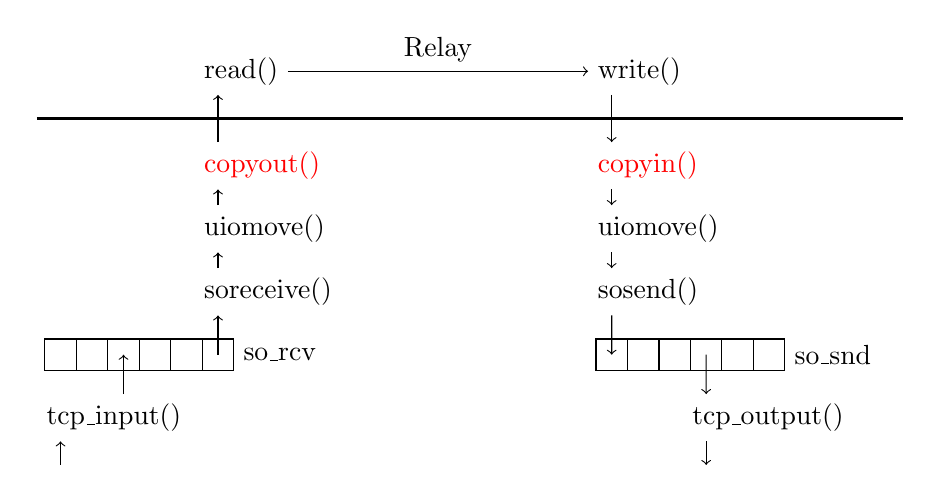
\begin{tikzpicture}
\draw (0,0)
    node (ti) [right] {tcp\_input()} ++(.1,.6)
    rectangle ++(.4,.4) rectangle ++(.4,-.4)
    rectangle ++(.4,.4) rectangle ++(.4,-.4)
    rectangle ++(.4,.4) rectangle ++(.4,-.4) ++(0,.2)
    node (rb) [right] {so\_rcv} ++(-.5,.8)
    node (sr) [right] {soreceive()} ++(0,.8)
    node (ur) [right] {uiomove()} ++(0,.8)
    node (co) [right,red] {copyout()} ++(0,1.2)
    node (rd) [right] {read()} ++(5,0)
    node (wr) [right] {write()} ++(0,-1.2)
    node (ci) [right,red] {copyin()} ++(0,-.8)
    node (us) [right] {uiomove()} ++(0,-.8)
    node (ss) [right] {sosend()} ++(.1,-.6)
    rectangle ++(.4,-.4) rectangle ++(.4,.4)
    rectangle ++(.4,-.4) rectangle ++(.4,.4)
    rectangle ++(.4,-.4) rectangle ++(.4,.4) ++(0,-.2)
    node (sb) [right] {so\_snd} ++(-1.3,-.8)
    node (to) [right] {tcp\_output()};

\path (node cs:name=ti,anchor=west) +(.3,-.3) coordinate (tii) {};
\draw[->] (tii) +(0,-.3) -- (tii);
\path (node cs:name=ti,anchor=west) +(.3+2*.4,.3) coordinate (tio) {};
\path (node cs:name=rb,anchor=west) +(-.2-3*.4,0) coordinate (rbi) {};
\draw[->] (tio) -- (rbi);
\path (node cs:name=rb,anchor=west) +(-.2,0) coordinate (rbo) {};
\path (node cs:name=sr,anchor=west) +(.3,-.3) coordinate (sri) {};
\draw[->] (rbo) -- (sri);
\path (node cs:name=sr,anchor=west) +(.3,.3) coordinate (sro) {};
\path (node cs:name=ur,anchor=west) +(.3,-.3) coordinate (uri) {};
\draw[->] (sro) -- (uri);
\path (node cs:name=ur,anchor=west) +(.3,.3) coordinate (uro) {};
\path (node cs:name=co,anchor=west) +(.3,-.3) coordinate (coi) {};
\draw[->] (uro) -- (coi);
\path (node cs:name=co,anchor=west) +(.3,.3) coordinate (coo) {};
\path (node cs:name=rd,anchor=west) +(.3,-.3) coordinate (rdi) {};
\draw[->] (coo) -- (rdi);
\draw[->] (node cs:name=rd,anchor=east) -- node [above] {Relay}
    (node cs:name=wr,anchor=west);
\path (node cs:name=wr,anchor=west) +(.3,-.3) coordinate (wro) {};
\path (node cs:name=ci,anchor=west) +(.3,.3) coordinate (cii) {};
\draw[->] (wro) -- (cii);
\path (node cs:name=ci,anchor=west) +(.3,-.3) coordinate (cio) {};
\path (node cs:name=us,anchor=west) +(.3,.3) coordinate (usi) {};
\draw[->] (cio) -- (usi);
\path (node cs:name=us,anchor=west) +(.3,-.3) coordinate (uso) {};
\path (node cs:name=ss,anchor=west) +(.3,.3) coordinate (ssi) {};
\draw[->] (uso) -- (ssi);
\path (node cs:name=ss,anchor=west) +(.3,-.3) coordinate (sso) {};
\path (node cs:name=sb,anchor=west) +(-.2-5*.4,0) coordinate (sbi) {};
\draw[->] (sso) -- (sbi);
\path (node cs:name=sb,anchor=west) +(-.2-2*.4,0) coordinate (sbo) {};
\path (node cs:name=to,anchor=west) +(.3,.3) coordinate (toi) {};
\draw[->] (sbo) -- (toi);
\path (node cs:name=to,anchor=west) +(.3,-.3) coordinate (too) {};
\draw[->] (too) -- +(0,-.3) ;

\draw[thick] (rdi -| 0,0) ++(0,-.3) node (context) {} -- +(11,0);
\end{tikzpicture}
\end{frame}

\begin{frame}{Process Wakeup}
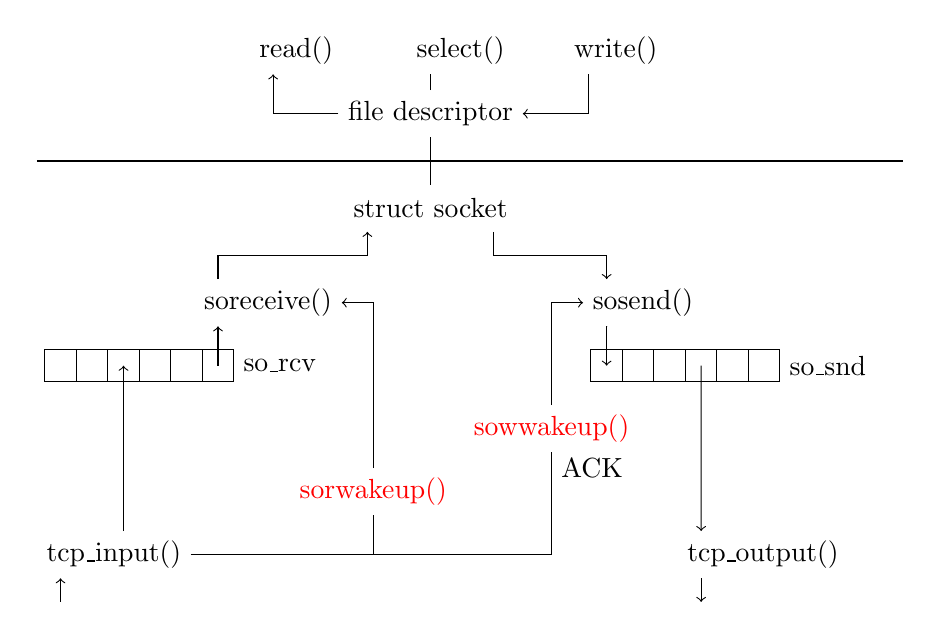
\begin{tikzpicture}
\draw (0,0)
    node (ti) [right] {tcp\_input()} ++(.1,2.2)
    rectangle ++(.4,.4) rectangle ++(.4,-.4)
    rectangle ++(.4,.4) rectangle ++(.4,-.4)
    rectangle ++(.4,.4) rectangle ++(.4,-.4) ++(0,.2)
    node (rb) [right] {so\_rcv} ++(-.5,.8)
    node (sr) [right] {soreceive()} ++(3,1.2)
    node (so) {struct socket} ++(0,1.2)
    node (fd) {file descriptor} +(-2-.3,.8)
    node (rd) [right] {read()} +(-.3,.8)
    node (sl) [right] {select()} +(2-.3,.8)
    node (wr) [right] {write()};
\draw (sr) ++(4,0)
    node (ss) [right] {sosend()} ++(.1,-.6)
    rectangle ++(.4,-.4) rectangle ++(.4,.4)
    rectangle ++(.4,-.4) rectangle ++(.4,.4)
    rectangle ++(.4,-.4) rectangle ++(.4,.4) ++(0,-.2)
    node (sb) [right] {so\_snd} ++(-1.3,-2.4)
    node (to) [right] {tcp\_output()};

\path (node cs:name=ti,anchor=west) +(.3,-.3) coordinate (tii) {};
\draw[->] (tii) +(0,-.3) -- (tii);
\path (node cs:name=ti,anchor=west) +(.3+2*.4,.3) coordinate (tio) {};
\path (node cs:name=rb,anchor=west) +(-.2-3*.4,0) coordinate (rbi) {};
\draw[->] (tio) -- (rbi);
\path (node cs:name=rb,anchor=west) +(-.2,0) coordinate (rbo) {};
\path (node cs:name=sr,anchor=west) +(.3,-.3) coordinate (sri) {};
\draw[->] (rbo) -- (sri);
\path (node cs:name=sr,anchor=west) +(.3,.3) coordinate (sro) {};
\path (so) +(0,-.6) coordinate (sox) {};
\path (node cs:name=so,anchor=west) +(.3,-.3) coordinate (soi) {};
\draw[->] (sro) -- (sro |- sox) -| (soi);

\path (node cs:name=so,anchor=east) +(-.3,-.3) coordinate (soo) {};
\path (node cs:name=ss,anchor=west) +(.3,.3) coordinate (ssi) {};
\draw[->] (soo) -- (soo |- sox) -| (ssi);
\path (node cs:name=ss,anchor=west) +(.3,-.3) coordinate (sso) {};
\path (node cs:name=sb,anchor=west) +(-.2-5*.4,0) coordinate (sbi) {};
\draw[->] (sso) -| (sbi);
\path (node cs:name=sb,anchor=west) +(-.2-2*.4,0) coordinate (sbo) {};
\path (node cs:name=to,anchor=west) +(.3,.3) coordinate (toi) {};
\draw[->] (sbo) -- (toi);
\path (node cs:name=to,anchor=west) +(.3,-.3) coordinate (too) {};
\draw[->] (too) -- +(0,-.3);

\path (node cs:name=ti,anchor=east) coordinate (tiw) {};
\path (node cs:name=sr,anchor=east) coordinate (srw) {}
    +(.4,0) coordinate (srx) {};
\draw[->] (tiw) -- (tiw -| srx) -- ++(0,.5) ++(0,.3)
    node (rw) [red] {sorwakeup()} ++(0,.3) |- (srw);
\path (node cs:name=ss,anchor=west) coordinate (ssw) {}
    +(-.4,0) coordinate (ssx) {};
\draw[->] (tiw) -- (tiw -| ssx) -- ++(0,1.3)  ++(0,.3)
    node (ww) [red] {sowwakeup()} ++(0,.3) |- (ssw);
\draw (node cs:name=ww,anchor=south) ++(0,-.2) node [right] {ACK};

\path (node cs:name=rd,anchor=west) +(.3,-.3) coordinate (rdi) {};
\draw[->] (node cs:name=fd,anchor=west) -| (rdi);
\path (node cs:name=wr,anchor=west) +(.3,-.3) coordinate (wro) {};
\draw[->] (wro) |- (node cs:name=fd,anchor=east);
\path (node cs:name=sl,anchor=west) +(.3,-.3) coordinate (sli) {};
\draw (fd) +(0,+.3) -- (sli);

\path (so) +(0,.3) coordinate (soc) {};
\path (fd) +(0,-.3) coordinate (fdc) {};
\draw (soc) -- (fdc);
\draw[thick] (fdc -| 0,0) ++(0,-.3) node (context) {} -- +(11,0);
\end{tikzpicture}
\end{frame}

\section{Socket Splicing}

\begin{frame}{Agenda}
\tableofcontents[currentsection]
\end{frame}

\begin{frame}{Socket Splicing}
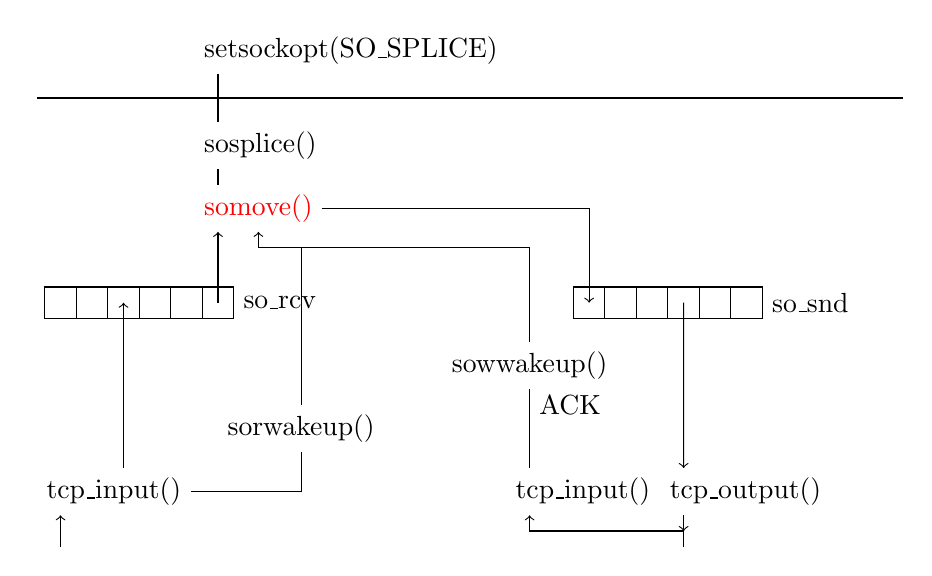
\begin{tikzpicture}
\draw (0,0)
    node (ti) [right] {tcp\_input()} ++(.1,2.2)
    rectangle ++(.4,.4) rectangle ++(.4,-.4)
    rectangle ++(.4,.4) rectangle ++(.4,-.4)
    rectangle ++(.4,.4) rectangle ++(.4,-.4) ++(0,.2)
    node (rb) [right] {so\_rcv} ++(-.5,1.2)
    node (sm) [right,red] {somove()} ++(0,.8)
    node (ss) [right] {sosplice()} ++(0,1.2)
    node (so) [right] {setsockopt(SO\_SPLICE)};
\draw (sm) ++(4,-1.0)
    rectangle ++(.4,-.4) rectangle ++(.4,.4)
    rectangle ++(.4,-.4) rectangle ++(.4,.4)
    rectangle ++(.4,-.4) rectangle ++(.4,.4) ++(0,-.2)
    node (sb) [right] {so\_snd} ++(-1.3,-2.4)
    node (to) [right] {tcp\_output()}
    node (ta) [left] {tcp\_input()};

\path (node cs:name=ti,anchor=west) +(.3,-.3) coordinate (tii) {};
\draw[->] (tii) +(0,-.4) -- (tii);
\path (node cs:name=ti,anchor=west) +(.3+2*.4,.3) coordinate (tio) {};
\path (node cs:name=rb,anchor=west) +(-.2-3*.4,0) coordinate (rbi) {};
\draw[->] (tio) -- (rbi);
\path (node cs:name=rb,anchor=west) +(-.2,0) coordinate (rbo) {};
\path (node cs:name=sm,anchor=west) +(.3,-.3) coordinate (smi) {};
\draw[->] (rbo) -- (smi);
\path (node cs:name=sm,anchor=west) +(.3,.3) coordinate (smo) {};
\path (node cs:name=ss,anchor=west) +(.3,-.3) coordinate (ssi) {};
\draw (smo) -- (ssi);
\path (node cs:name=ss,anchor=west) +(.3,.3) coordinate (sso) {};
\path (node cs:name=so,anchor=west) +(.3,-.3) coordinate (soi) {};
\draw (sso) -- (soi);

\path (node cs:name=sb,anchor=west) +(-.2-5*.4,0) coordinate (sbi) {};
\draw[->] (node cs:name=sm,anchor=east) -| (sbi);
\path (node cs:name=sb,anchor=west) +(-.2-2*.4,0) coordinate (sbo) {};
\path (node cs:name=to,anchor=west) +(.3,.3) coordinate (toi) {};
\draw[->] (sbo) -- (toi);
\path (node cs:name=to,anchor=west) +(.3,-.3) coordinate (too) {};
\path (too) +(0,-.2) coordinate (tx) {};
\draw[->] (too) -- (tx);

\path (sm) +(0,-.3) coordinate (smw) {} +(0,-.5) coordinate (smx) {};
\path (node cs:name=ta,anchor=west) +(.3,-.3) coordinate (tai) {};
\draw (node cs:name=ti,anchor=east) -| ++(1.4,.5) ++(0,.3)
    node (rw) {sorwakeup()} ++(0,.3) |- (smx);
\path (node cs:name=ta,anchor=west) +(.3,-.3) coordinate (tai) {};
\draw[->] (tx) +(0,-.2) -- (tx) -| (tai);
\path (node cs:name=ta,anchor=west) +(.3,.3) coordinate (tao) {};
\draw[->] (tao) -- ++(0,1)  ++(0,.3)
    node (ww) {sowwakeup()} ++(0,.3) |- (smx) -- (smw);
\draw (node cs:name=ww,anchor=south) ++(0,-.2) node [right] {ACK};

\draw[thick] (soi -| 0,0) ++(0,-.3) node (context) {} -- +(11,0);
\end{tikzpicture}
\end{frame}

\begin{frame}{UDP Sockets}
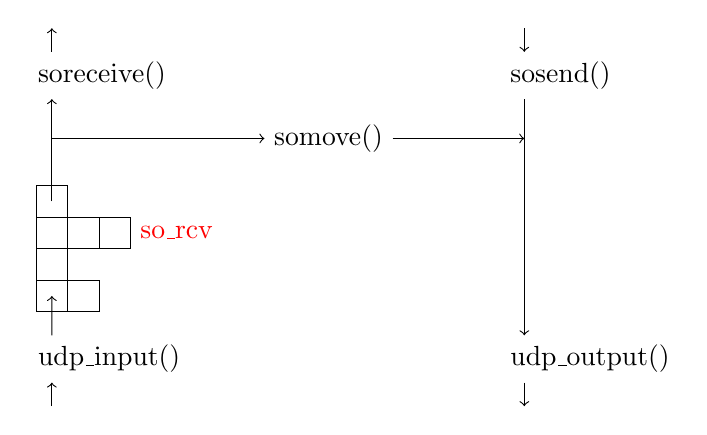
\begin{tikzpicture}
\draw (0,0)
    node (ui) [right] {udp\_input()} ++(.1,.6)
    rectangle ++(.4,.4) rectangle ++(.4,-.4) ++(-.8,.4)
    rectangle ++(.4,.4) ++(-.4,0)
    rectangle ++(.4,.4) rectangle ++(.4,-.4) rectangle ++(.4,.4) ++(0,-.2)
    node (rb) [right,red] {so\_rcv} ++(-3*.4,.2)
    rectangle ++(.4,.4) ++(-.5,.6+.8)
    node (sr) [right] {soreceive()} ++(3,-.8)
    node (sm) [right] {somove()} ++(3,.8)
    node (ss) [right] {sosend()} (node cs:name=ss,anchor=west)
    coordinate (ssw) {} (ssw |- ui)
    node (uo) [right] {udp\_output()};

\path (node cs:name=ui,anchor=west) +(.3,-.3) coordinate (uii) {};
\draw[->] (uii) +(0,-.3) -- (uii);
\path (node cs:name=ui,anchor=west) +(.3,.3) coordinate (uio) {};
\path (node cs:name=rb,anchor=west) +(-.2-2*.4,-.8) coordinate (rbi) {};
\draw[->] (uio) -- (rbi);
\path (node cs:name=rb,anchor=west) +(-.2-2*.4,.4) coordinate (rbo) {};
\path (node cs:name=sr,anchor=west) +(.3,-.3) coordinate (sri) {};
\draw[->] (rbo) -- (sri);
\path (node cs:name=sr,anchor=west) +(.3,.3) coordinate (sro) {};
\draw[->] (sro) -- +(0,.3);

\path (node cs:name=ss,anchor=west) +(.3,.3) coordinate (ssi) {};
\draw[->] (ssi) +(0,.3) -- (ssi);
\path (node cs:name=ss,anchor=west) +(.3,-.3) coordinate (sso) {};
\path (node cs:name=uo,anchor=west) +(.3,.3) coordinate (uoi) {};
\draw[->] (sso) -- (uoi);
\path (node cs:name=uo,anchor=west) +(.3,-.3) coordinate (uoo) {};
\draw[->] (uoo) -- +(0,-.3) ;

\path (node cs:name=sm,anchor=west) coordinate (smi) {};
\draw[->] (rbo |- smi) -- (smi);
\path (node cs:name=sm,anchor=east) coordinate (smo) {};
\draw[->] (smo) -- (smo -| uoi);

\end{tikzpicture}
\end{frame}

\begin{frame}{Layer}
\begin{tikzpicture}
\draw (0,0)
    rectangle ++(.4,.4) rectangle ++(.4,-.4)
    rectangle ++(.4,.4) rectangle ++(.4,-.4)
    rectangle ++(.4,.4) rectangle ++(.4,-.4) ++(0,.2)
    node (rq) [right] {ipintrq} ++(-.5-5*.4,.8)
    node (ii) [right] {ip\_input()} ++(0,.8)
    node (ti) [right] {tcp\_input()} ++(.1,.6)
    rectangle ++(.4,.4) rectangle ++(.4,-.4)
    rectangle ++(.4,.4) rectangle ++(.4,-.4)
    rectangle ++(.4,.4) rectangle ++(.4,-.4) ++(0,.2)
    node (rb) [right] {so\_rcv} ++(-.5,1.6)
    node (sr) [right] {soreceive()} ++(0,1.2)
    node (rd) [right] {read()} ++(5,0)
    node (wr) [right] {write()} ++(0,-1.2)
    node (ss) [right] {sosend()} ++(.1,-1.4)
    rectangle ++(.4,-.4) rectangle ++(.4,.4)
    rectangle ++(.4,-.4) rectangle ++(.4,.4)
    rectangle ++(.4,-.4) rectangle ++(.4,.4) ++(0,-.2)
    node (sb) [right] {so\_snd} ++(-.3-.2-5*.4,-.8)
    node (to) [right] {tcp\_output()} ++(0,-.8)
    node (io) [right] {ip\_output()} ++(.1,-.6)
    rectangle ++(.4,-.4) rectangle ++(.4,.4)
    rectangle ++(.4,-.4) rectangle ++(.4,.4)
    rectangle ++(.4,-.4) rectangle ++(.4,.4) ++(0,-.2)
    node (sq) [right] {if\_snd} ++(-.5,-.8);

\path (node cs:name=rq,anchor=west) +(-.2-5*.4,0) coordinate (rqo) {};
\path (node cs:name=ii,anchor=west) +(.3,-.3) coordinate (iii) {};
\draw[->] (rqo) -- (iii);
\path (node cs:name=ii,anchor=west) +(.3,.3) coordinate (iio) {};
\path (node cs:name=ti,anchor=west) +(.3,-.3) coordinate (tii) {};
\draw[->] (iio) -- (tii);
\path (node cs:name=ti,anchor=west) +(.3+2*.4,.3) coordinate (tio) {};
\path (node cs:name=rb,anchor=west) +(-.2-3*.4,0) coordinate (rbi) {};
\draw[->] (tio) -- (rbi);
\path (node cs:name=rb,anchor=west) +(-.2,0) coordinate (rbo) {};
\path (node cs:name=sr,anchor=west) +(.3,-.3) coordinate (sri) {};
\draw[->] (rbo) -- (sri);
\path (node cs:name=sr,anchor=west) +(.3,.3) coordinate (sro) {};
\path (node cs:name=rd,anchor=west) +(.3,-.3) coordinate (rdi) {};
\draw[->] (sro) -- (rdi);
\draw[->] (node cs:name=rd,anchor=east) -- node [above] {Relaying}
    (node cs:name=wr,anchor=west);
\path (node cs:name=wr,anchor=west) +(.3,-.3) coordinate (wro) {};
\path (node cs:name=ci,anchor=west) +(.3,.3) coordinate (cii) {};
\path (node cs:name=ss,anchor=west) +(.3,.3) coordinate (ssi) {};
\draw[->] (wro) -- (ssi);
\path (node cs:name=ss,anchor=west) +(.3,-.3) coordinate (sso) {};
\path (node cs:name=sb,anchor=west) +(-.2-5*.4,0) coordinate (sbi) {};
\draw[->] (sso) -- (sbi);
\path (node cs:name=sb,anchor=west) +(-.2-2*.4,0) coordinate (sbo) {};
\path (node cs:name=to,anchor=west) +(.3+3*.4,.3) coordinate (toi) {};
\draw[->] (sbo) -- (toi);
\path (node cs:name=to,anchor=west) +(.3,-.3) coordinate (too) {};
\path (node cs:name=io,anchor=west) +(.3,.3) coordinate (ioi) {};
\draw[->] (too) -- (ioi);
\path (node cs:name=io,anchor=west) +(.3,-.3) coordinate (ioo) {};
\path (node cs:name=sq,anchor=west) +(-.2-5*.4,0) coordinate (sqi) {};
\draw[->] (ioo) -- (sqi);

\draw[->] (node cs:name=ii,anchor=east) -- node [above] {Forwarding}
    (node cs:name=io,anchor=west);
\path (sri) +(0,-.8) coordinate (srx) {};
\path (sso) +(0,-.8) coordinate (ssx) {};
\draw[->] (srx) -- node [above,red] {Socket Splicing} (ssx);

\draw[thick] (rdi -| 0,0) ++(0,-.3) node (context) {} -- +(11,0);
\end{tikzpicture}
\end{frame}

\section{Interface}

\begin{frame}{Agenda}
\tableofcontents[currentsection]
\end{frame}

\begin{frame}{Simple API}
\begin{itemize}
    \item Begin splicing from source to drain\\
	setsockopt(source\_fd, SO\_SPLICE, drain\_fd)
    \item Stop splicing\\
	setsockopt(source\_fd, SO\_SPLICE, -1)
    \item Get spliced data length\\
	getsockopt(source\_fd, SO\_SPLICE, \&length)
\end{itemize}
\end{frame}

\begin{frame}[fragile]{Extended API}
\begin{verbatim}
struct splice {
  int    sp_fd;           /* drain */
  off_t  sp_max;          /* maximum */
  struct timeval sp_idle; /* timeout */
};
\end{verbatim}
setsockopt(source\_fd, SO\_SPLICE, \&splice)
\end{frame}

\begin{frame}{Properties}
\begin{itemize}
    \item Splicing is unidirectional
    \item Invoke it twice for bidirectional splicing
    \item Process can turn it on and off
    \item Works for TCP and UDP
    \item Can mix IPv4 and IPv6 sockets
\end{itemize}
\end{frame}

\begin{frame}{Unsplice}
\begin{itemize}
    \item Dissolve socket splicing manually
    \item read(2) or select(2) from the source
    \item EOF source socket shutdown
    \item EPIPE drain socket error
    \item EFBIG maximum data length
    \item ETIMEDOUT idle timeout
\end{itemize}
\end{frame}

\section{Implementation}

\begin{frame}{Agenda}
\tableofcontents[currentsection]
\end{frame}

\begin{frame}[fragile]{Struct Socket}
\begin{verbatim}
struct socket {
    ...
    struct  socket *so_splice;
    struct  socket *so_spliceback;
    off_t   so_splicelen;
    off_t   so_splicemax;
    struct  timeval so_idletv;
    struct  timeout so_idleto;
    ...
};
\end{verbatim}
\end{frame}

\begin{frame}{sosplice(9)}
\begin{itemize}
    \item Protocol must match
    \item Sockets must be connected
    \item Double link sockets
    \item Move existing data
\end{itemize}
\end{frame}

\begin{frame}{somove(9)}
\begin{itemize}
    \item Check for errors
    \item Check for space
    \item Handle maximum
    \item Handle out of band data
    \item Move socket buffer data
\end{itemize}
\end{frame}

\begin{frame}{sounsplice()}
\begin{itemize}
    \item Manual unsplice
    \item Cannot receive
    \item Cannot send
    \item Maximum
    \item Timeout
    \item Socket closed
\end{itemize}
\end{frame}

\begin{frame}{sorwakeup() sowwakeup()}
\begin{itemize}
    \item Called from tcp\_input()
    \item Source calls sorwakeup()
    \item Drain calls sowwakeup()
    \item Both invoke somove(9)
\end{itemize}
\end{frame}

\section{Applications}

\begin{frame}{Agenda}
\tableofcontents[currentsection]
\end{frame}

\begin{frame}{Relayd}
\begin{itemize}
    \item Plain TCP connections
    \item HTTP connections
    \item Filter persistent HTTP
    \item HTTP Chunking
\end{itemize}
\end{frame}

\begin{frame}{Tests}
\begin{itemize}
    \item /usr/src/regress/sys/kern/sosplice/
    \item 15 API tests
    \item 18 UDP tests
    \item 76 TCP tests
    \item perf/relay.c simple example
    \item BSD::Socket::Splice Perl API
    \item 28 relayd tests
\end{itemize}
\end{frame}

\begin{frame}{Performance}
\begin{itemize}
    \item Factor 1 or 2 for TCP
    \item Factor 6 or 8 for UDP
\end{itemize}
\end{frame}

\begin{frame}{Documentation}
\begin{itemize}
    \item Manpage setsockopt(2) SO\_SPLICE
    \item Manpage sosplice(9) somove(9)
\end{itemize}
\end{frame}

\begin{frame}{Questions}
\begin{center}
\begin{tikzpicture}
\draw [font=\fontsize{6cm}{4cm}\selectfont] node {?};
\end{tikzpicture}
\end{center}
\end{frame}

\end{document}
